\documentclass{article}
\usepackage[utf8x]{inputenc}
\usepackage{float}
\usepackage{graphics}
\usepackage{graphicx}
\usepackage[colorlinks,pdfpagelabels,pdfstartview = FitH,bookmarksopen = true,bookmarksnumbered = true,linkcolor = black,plainpages = false,hypertexnames = false,citecolor = black] {hyperref}

\begin{document}
\begin{titlepage}
 
%opening

\newcommand{\changefont}[3]{
\fontfamily{#1}  \fontseries{#2}  \fontshape{#3}  \selectfont}

\title{\huge \textbf{S.C.O.R.E  MyCourses} \vskip 2ex 
\includegraphics[width=0.5\textwidth]{images/scetris_trans_blackglow.png} \vskip 2ex \textbf{\large Summary report} \vskip 2ex}
\author{\changefont{cmr}{m}{sc} David Bialik, Julian Fleischer, Hagen Mahnke,\\ \changefont{cmr}{m}{sc} Konrad Reiche, André Zoufahl}
\date{\today}

\maketitle

\vskip 3ex
\center 
\includegraphics[width=0.3\textwidth]{images/siegel.jpg}

\center \changefont{cmr}{m}{sc} \LARGE Free University of Berlin \vskip 2ex \large Department of Mathematics and Computer Science\\Institute of Computer Science

\thispagestyle{empty}
\end{titlepage}

\newpage

\tableofcontents

\newpage

\begin{abstract}
This document summarizes the activities of a team of undergraduate students participating in the student contest on software engineering [SCORE] 2011. The carried out project was myCourses. (The work was done on the project myCourses.) The document contains descriptions of the work done during the development process. In particular about the requirement solicitation, requirements specification, design and the implementation. (It provides a description of the problem, the software development process and the product.)
\end{abstract}





\section{Who we are}

We are a team of five undergraduate students of the Free University of Berlin. Even though  we are all in the same year our knowledge regarding the creation of software and the used technologies varied widely. We were however all inexperienced in project management. Specifically none of us had been part of a software development process before. The members of the team, their age and their most prominent task are:
\begin{itemize}
	\item David Bialik, 23, build automatization, installer
	\item Julian Fleischer, 23, backend development
	\item Hagen Mahnke, 24, project lead
	\item Konrad Reiche, 22, scheduler development
	\item Andre Zoufahl, 22, web interface development
\end{itemize}

\begin{figure}[H]
	\centering
		
\includegraphics[width=\textwidth]{images/CROWD.png}
	\caption{\small From left to right: David Bialik, Konrad Reiche, Hagen Mahnke, Julian Fleischer, Andre Zoufahl, Mister X}
	\label{fig:us}
\end{figure}



\section{Development process}
In the following two sections our development process will be described and reviewed. The first section is a description of our initial ideas and the rationale behind it. The second section describes how our development process actually happened and where we altered it.

\subsection{Intended development process}
As mentioned before the team lacked experience in projects but we knew a bit of software engineering theory. We all agreed that a perfect evaluation of requirements and creation of an appropriate plan was very unlikely. The reasoning for this assumption is again our lack of experience. On the other hand we also saw need for as much structure as we could sensibly apply. This assumption is based on us not working full-time and conducting most of our work isolated. Thus we decided to use an iterative model, expecting many revisions of earlier assessments. To be more precise we decided to follow the spiral model. We expected the structure of defined iterations and tasks for these iterations to compensate our lack of experience in planning. Of course we did not plan to rely blindly on the model to define our process. We rather chose the spiral model as the basis for our own process and assumed that adaption would become necessary. We did not however have a clear concept of what might require adaption and how said adaption might be realized.

\vskip 2ex

When deciding to follow the spiral model we also planned for risk management and quality assurance phases in every iteration. However we missed the fact that the most important aspect of the spiral model is risk management. How exactly this went unnoticed is not clear, but in the result we planned less risk management than appropriate for a spiral model.

\vskip 2ex

Key components of our process were
\begin{itemize}
	\item regular meetings for coordination
	\item communication through e-mail
	\item evaluation of iterations
	\item ticket system for definition and monitoring of tasks
	\item wiki for shared documents
\end{itemize}

\subsection{Actual development process}
As we expected some of our initial ideas were unsuitable or even obstructive. The following paragraphs will discuss where we adhered to our initial plan and where we did not, as well as evaluate our decisions or lack thereof.

\vskip 2ex

As intended we held regular meetings with the whole team to discuss what has been achieved, what could be improved and how the time until the next meeting will be spend. These meetings addressed mostly organizational issues but design and implementation were also discussed. From the end of May until the beginning of October meetings were held on a two-weeks basis. Within our third iteration in October we picked up the frequency and met weekly. This change is due to  integration of parts of our systems with each other, increasing necessity for coordination. We kept meeting weekly thereafter as we found the interval to be fitting our work-cycles well. Due to our workload and our need for orientation at the start we doubt that a weekly cycle would have been appropriate right away. However we could have benefited from starting to meet weekly in August. At that time we often met several days in a row but used it for coding and did neither define nor evaluate tasks clearly. All the time we invested in August and September might have been used more efficient, had we taken the time to review each week.

\vskip 2ex

E-mail was our main medium of communication throughout almost the whole process. As we all study at the same university  this choice might be surprising. Despite living in relative proximity to each other and meeting often at the university, the times we could meet to work on the project were few. Thus an asynchronous communication was a natural choice. A mailing-list was used for organizational issues as well as for artifact related topics. All e-mails were sent to the list even if they were aimed at a single or few receivers. The assumption was that reading e-mails on all the topics would help distributing knowledge to the whole team. On the other hand the high amount of e-mails posed a significant amount of work if read thoroughly. One might also argue that reading isolated informations about topics does not work very well for passive knowledge transfer, so the positive effect might be even smaller. Another problem of our communication was the tendency to mix several unrelated messages into a single e-mail. As a result everyone was forced to read every mail at least fleetingly. Even worse information could sometimes not be found a few weeks later. A clear separation was attempted several times but we failed to adhere to it.

\vskip 2ex 

We did evaluate our iterations at their end and attempted to find weaknesses as well as ways to improve upon them. Positive aspects were discussed as well to gain a more balanced perspective of how we were doing. However success of our evaluations has been moderate as problems, when identified, were tackled ineffectively. On the other hand we did improve upon our process and the execution of it. We just did it whenever someone, often a group of people, noticed something amiss and informed the others. In all cases a discussion ensued and ended in decisions that were far better respected than the ones obtained during official evaluations. We assume this is due to the swift dealing with real problems, leaving only minor or even purely perception based problems for evaluation. We kept evaluating nonetheless as it was a good opportunity for giving feedback.

\vskip 2ex

We decided to use a trac system providing us with tickets and a wiki. Both were used to coordinate the assignment of tasks and gather information about progress and possible problems. The usage of the ticket system was minimal in the beginning and only picked up later, leading to a conducive usage from October. This is also one of the examples where a problem was informally addressed by a member followed by a significant improvement. Prior to this point the problem had been minor, as almost all the work had been done with most of the team present.

During the process we noticed that the spiral model was not flexible enough for our needs and most likely requires more experience than we had. For example we were unable to provide good estimations for amount and time of work and our iterations were actually far too long. Thus we consecutively changed our process, leading to
\begin{itemize}
	\item shorter work-cycles
	\item mostly informal evaluation and feedback
	\item very little risk-management 
\end{itemize}

Regarding risk-management we planned to have a special phase in each iteration dedicated to evaluation and risk-management. During the project we experienced that we did not fully understand how risk-management can be achieved. Our main problem with this point was the lack of good criteria to decide what it means to fail a certain aspect and what an appropriate counter-measure is. For example it could be clear to us that a certain module could not fail, for else the project would fail. Now it would have been necessary to develop a precise plan of action for each point at which said module might fail. What happened however was that people had vague ideas about a certain course of action but not more. This lead to an all but complete abandoning of risk-management.

\subsection{Timeline}
A short overview of the course our project took will be given in the next paragraphs. The goals for a phase were defined after evaluation of the previous phase was completed. Before our project really started we got to know each other and decided which professor should be our contact person at the university.

\begin{description}
\item[First iteration] started on June 20 and comprised of an initial requirement elicitation, design of our software, prototyping of the scheduler and choosing technologies. During most of this time the academic term was still running and only a fraction of our time was devoted to the project. This iteration ended on September 9 and was evaluated the day before. Much of the time spent in this iteration was still focused on gaining orientation. Still it was necessary for us to take this time and find a suitable approach to the work ahead.

\item[Second iteration] started on September 10 and was devoted to producing the scheduling-algorithm, the web-interface and our ORM as well as weave and bakery. Work cycles were short and meetings were held every few days, including a weekend  devoted to coding. From this point on our iterations were reduced to about one month each and the focus was on implementing and testing. Requirements and design were refactored whenever we felt the need to due to new insights or problems. This iteration ended on October 4 and was evaluated the same day.

\item[Third iteration] accordingly started on October 5 but most work was halted until October 16 due to exams and all-day courses at university. Beginning with October 26 weekly two-hour meetings were held at our university in which everyone reported achievements and problems of the last week, as well as set goals for the next week. These weekly meetings have proven to be a good way of coordinating work as well as motivate each other, so they were conducted for the remainder of the project. The main goal and achievement of this iteration was the integration of the scheduler with the web-interface and the connection to the database. Due to this employment of parts of our software many issues were found and fixed. Accordingly we shifted our focus further towards unit-testing and started using a tool to measure code coverage, that is how much of our code is actually being executed  as part of a unit-test. At the same time more  functionality was added to the web-interface. This iteration ended on November 1 and was evaluated the day before.

\item[Fourth iteration] started on November 2 and was primarily focused on the improvement of our web-interface, adding functionality and a unified design. Some improvements to the scheduler-algorithm were made, most notably the introduction of a greedy-algorithm for the set up of the initial population. Work on the Summary Report was also started in this iteration and the first version which was the basis for all further versions was written. The iteration ended on December 5.

\item[Fifth iteration] started on December 6 and was mainly devoted to minor improvements to the scheduler and writing the beta-version of our summary report. One improvement to our database-access-layer which made query-caching available drastically improved scheduling performance by a factor of 8.
\end{description}
\section{Requirements}
The next two sections are a overview of the problem and the resulting requirements. The first section will state the problem, while the second describes the specification we deduced from it.

\subsection{Problem Statement}
Organizations like universities and schools are required to allocate courses to the given resources in a sensible way. As the amount of resources and courses grows large, it gets increasingly costly to do the allocation manually. Furthermore the task is repeated quite often and thus a lot of work is spent for it. Often the courses and resources remain similar each term and much of the previous solution can be reused. Each solution to such a problem must satisfy a number of constraints. These constraints often are, but are not limited to:
\begin{itemize}
	\item a room can only be booked once at a given time
	\item a lecturer can only lecture one course at a given time
	\item the different instances of a course must be held at different times
\end{itemize}
We called them hard-constraints.Furthermore a number of constraints exist that represent a preference. These constraints should be satisfied where possible but they need not be. These were called soft-constraints.

\subsection{Requirement elicitation}
Most of the requirements are already present in the project description of myCourses. While the need to find the requirements was mostly eliminated it is still helpful to be a more specific about the meaning of these requirements. To make the requirements more specific and better understood we created use-cases. These use-cases helped during implementation as the question of their realization was possible.

\vskip2ex

As we also desired more insight in how a scheduling process may look like, we asked an employee of our institute to give us a demonstration. The demonstration was conducted on the system used at our institute. While it did not reveal  completely unknown aspects to us it gave us a better estimation of the importance of certain aspects.

\subsection{Requirement specification}
The ideal scenario is a program that automatically finds an optimal solution. However the problem is NP-hard and thus a computer-aided scheduling process is the focus. As the interests of many employees and students at the universities are affected by the result, they should be allowed to participate in the process or at least be taken into consideration. The requirements that struck us as most important are the following:
\begin{itemize}
	\item automatic course allocation
	\item satisfaction of hard- and soft-constraints
	\item chance for manual allocations
	\item suited for multi-user environments
	\item scalable scheduling
	\item configurable system
	\item scheduling-related information is available
	\item definition of scheduling-related information is possible
	\item comfortable presentation to the user
	\item restricted access to information
\end{itemize}
These are the requirements that had the highest influence on our initial design and each subsequent change.


\section{Architectural design}

Many areas of our project required decisions and a rationale behind it. These decisions are sorted by area below and each decision is explained shortly. In retrospect some of these decisions were less than optimal while others turned out great and a description of how these influenced our project and what we learned will be given. The first section consists of a short overview of the system and a graphic representation. The second section talks about our database-access-layer. The third section talks about our web-framework. The fourth section is about a collection of tools for automatic code generation. The last section describes the scheduler algorithm.

\subsection{Overview}
Our system is best understood as a web-application providing the functionality to access the automatic solver and manipulate the data related to scheduling... 

\begin{figure}[H]
	\centering
		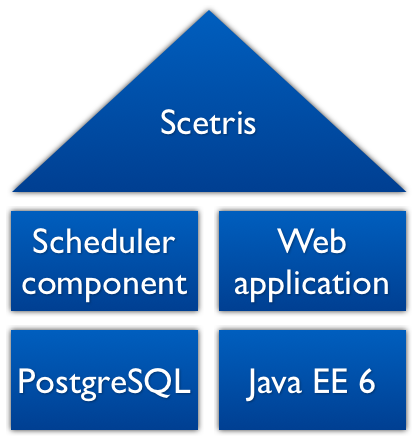
\includegraphics[width=0.5\textwidth]{images/scetris-house.png}
	\caption{\small An overview of the components}
	\label{fig:scetris-house}
\end{figure}

\subsection{Database access layer}

\emph{No existing solution but our own as we felt that existing solutions would take a similar amount of time to get used to and we would learn far more implementing the ORM ourselves. In regard to future work on the program, whether for maintenance or extension, it might prove beneficial to replace this solution with a more widely used tool, such as Hibernate. This would improve the process of understanding our software for people familiar with said tool. However we are satisfied with our own solution and we will stick with it, as it would be far too time-consuming to refactor this part of our project and we do not plan to work extensively with the software later on.}



\subsection{Web-framework}

\emph{Why we decided to use our own framework and how it is implemented. What the advantages are.}

We decided to implement our own web-framework as we wanted an easy integration of web-application and scheduling-algorithm. Thus a web-framework that uses the same language as our scheduling-algorithm was written to simplify the most common tasks. As well as getting a framework that fits our needs nicely, the benefit for us personally, which comes as knowledge was part of the reasoning against using an existing framework. We assume here that the knowledge of general principles is more beneficial to us than knowledge of tools.

\subsection{Tools for automatic code-generation}

\emph{Why a framework for common tasks has been created and how it affected our development process.}

As many tasks regarding the functionality of our web-interface require similar methods and should be implemented in a unified way to ease understanding, a framework for the most common tasks was written. It is called meta and is completely separated from the rest of our project, thus it can and will be used after we finished this project. So not only did it ease the development process for this project but also it will pay of even more in the long run.

\subsection{Scheduler Algorithm}
The problem of course scheduling is known to be NP-hard. The course scheduling problem can be approached by using search algorithms. As a matter of fact this works only for simple cases. Course scheduling, especially at universites and similiar big facilities, is faced with complex constraints. With the rise of input and more constraints finding an optimal solution cannot be computed in a sufficiently fast time. Based on several papers the approach of using a genetic algorithm is famous, seemed to be promising and was chosen therefore.

Genetic algorithm is a subset of metaheuristic optimization algorithm. Metaheuristics, being part of stochastic optimization, are algorithms using to some degree randomness in order to find optimal or as optimal as possible solutions to hard problems. Metaheuristics are applied when there is little to know about how the optimal solution looks like, there are to little heuristics to search on and brute-force is not questionable as the space of possible solution is to big. However when a candidate solution is given it can be scored in order to evaluate how good it is.

Typically a population of $\lambda$ number candidate solution is generated randomly, named \emph{setup}. The next step is an iteration containing the following process:

\begin{enumerate}
\item scoring the candidate solution by means of their \emph{fitness}

\item keeping only the $\mu$ best candidate solutions

\item generating new candidate solutions

	\begin{enumerate}
	\item selecting a candidate solution
	\item \emph{cross} it \emph{over} with another candidate solution
	\item \emph{mutate} the candidate solution
	\end{enumerate}
\end{enumerate}

To understand the the scheduler algorithm the genetic algorithm operations, \emph{setup}, \emph{fitness function}, \emph{crossover}, \emph{mutate} and \emph{selection} are best understood in means of core components of the scheduler algorithm. These operations are described below.

\begin{description}
\item[Setup] generates the initial population of candidate solutions in a random or semi-random way. A candidate solution is created when every course is allocated in a room at a given time. The \emph{setup} process is finished when $\lambda$ candidate solutions were created.

\item[Fitness function] evaluates the candidate solution by scoring it. The score is mapped to the number of constraints satisfied. The more constraints are satisfied the higher the candidate solution is scored. The score reaches from $0.0$ to $1.0$.

\item[Crossover] creates a new candidate solution by mixing and matching parts of two given candidate solution. How the mixing and matching is done relies on the representation of a candidate solution. As our representation is a mapping from courses to allocated room and time, these allocations are mixed and matched.

\item[Mutation] creates a new candidate solution by taking a given candidate solution and changing a specified amount of course allocations to new, randomly chosen, course allocations.

\item[Selection] iterates the given candidate solutions and keeps only the $\mu$ best solutions. The solutions are selected, according to the score given by the \emph{fitness function}, through dropping the rest of the candidate solutions.
\end{description}

The problem of course scheduling is defined by the given constraints which have to be satisfied. In order to meet the MyCourses specification requirements of high configurability we distinguish constraints by \emph{hard} and \emph{soft constraints}.

\begin{description}
\item[Hard constraints] are constraints which have to be satisfied. If these constraints are not satisfied the lecturing of courses is not possible. This includes the following constraints:

\begin{itemize}
\item not more than 1 course in the same room at the same time

\item the course lecturer has no other course at the same time

\item courses belonging to the same year do not overlap with each other in time in order to guarantee studiability

\item every constraint defined by the user with the priority of $100\%$, for instance preferred time, preferred room, etc.
\end{itemize}

\item[Soft constraints] are constraints which do not have to be ultimately satisfied. This includes only constraints defined by the user with a priority less than $100\%$.
\end{description}

An \emph{optimal solution} is a scheduling which asserts the satisfaction of all \emph{hard} and \emph{soft} constraints. Respectively the schedules score for \emph{hard} and \emph{soft fitness} is both $1.0$.

In the implementation phase it turned out using a \emph{setup} allocating the course completely random works for little input very well. With increased input, however, the results by  the classical \emph{setup} lead to quiet worse results. These results are supposed to be optimized by the phase of applying \emph{crossover} and \emph{mutate}. As a matter of fact this happens to a certain degree but starts to converging to a certain score.

Therefore an alternative \emph{setup} was implemented. \emph{Greedy setup} combines the approach of a genetic algorithm using metaheuristic with the Greedy algorithm being a subset of the combinatorial algorithm.

\begin{description}
\item[Greedy Setup] generates the initial population of candidate solutions by using a Greedy algorithm. Every course is allocated by placing it to the room which fits its constraints the best, for instance the requirement for a specified amount of seats. In order to avoid choosing rooms which exceed the required constraints every room is scored and sorted. In order to avoid overlapping in space and time the courses are place one after another in the timetable.
\end{description}

Figure \ref{fig:scheduler} illustrates the components interaction. At the start of each scheduling a initial population containing $\lambda$ possible schedule solutions is generated by \emph{Greedy Setup}. Randomly chosen courses are placed into the room which fits the course constraints the best. In this step the time slots are chosen at the earliest possible time slot and are distributed along all days at the week. If, however, there is a constraint for a preferred room or a preferred time slot entered by the user this spot is chosen directly.

\begin{figure}[H]
	\centering
		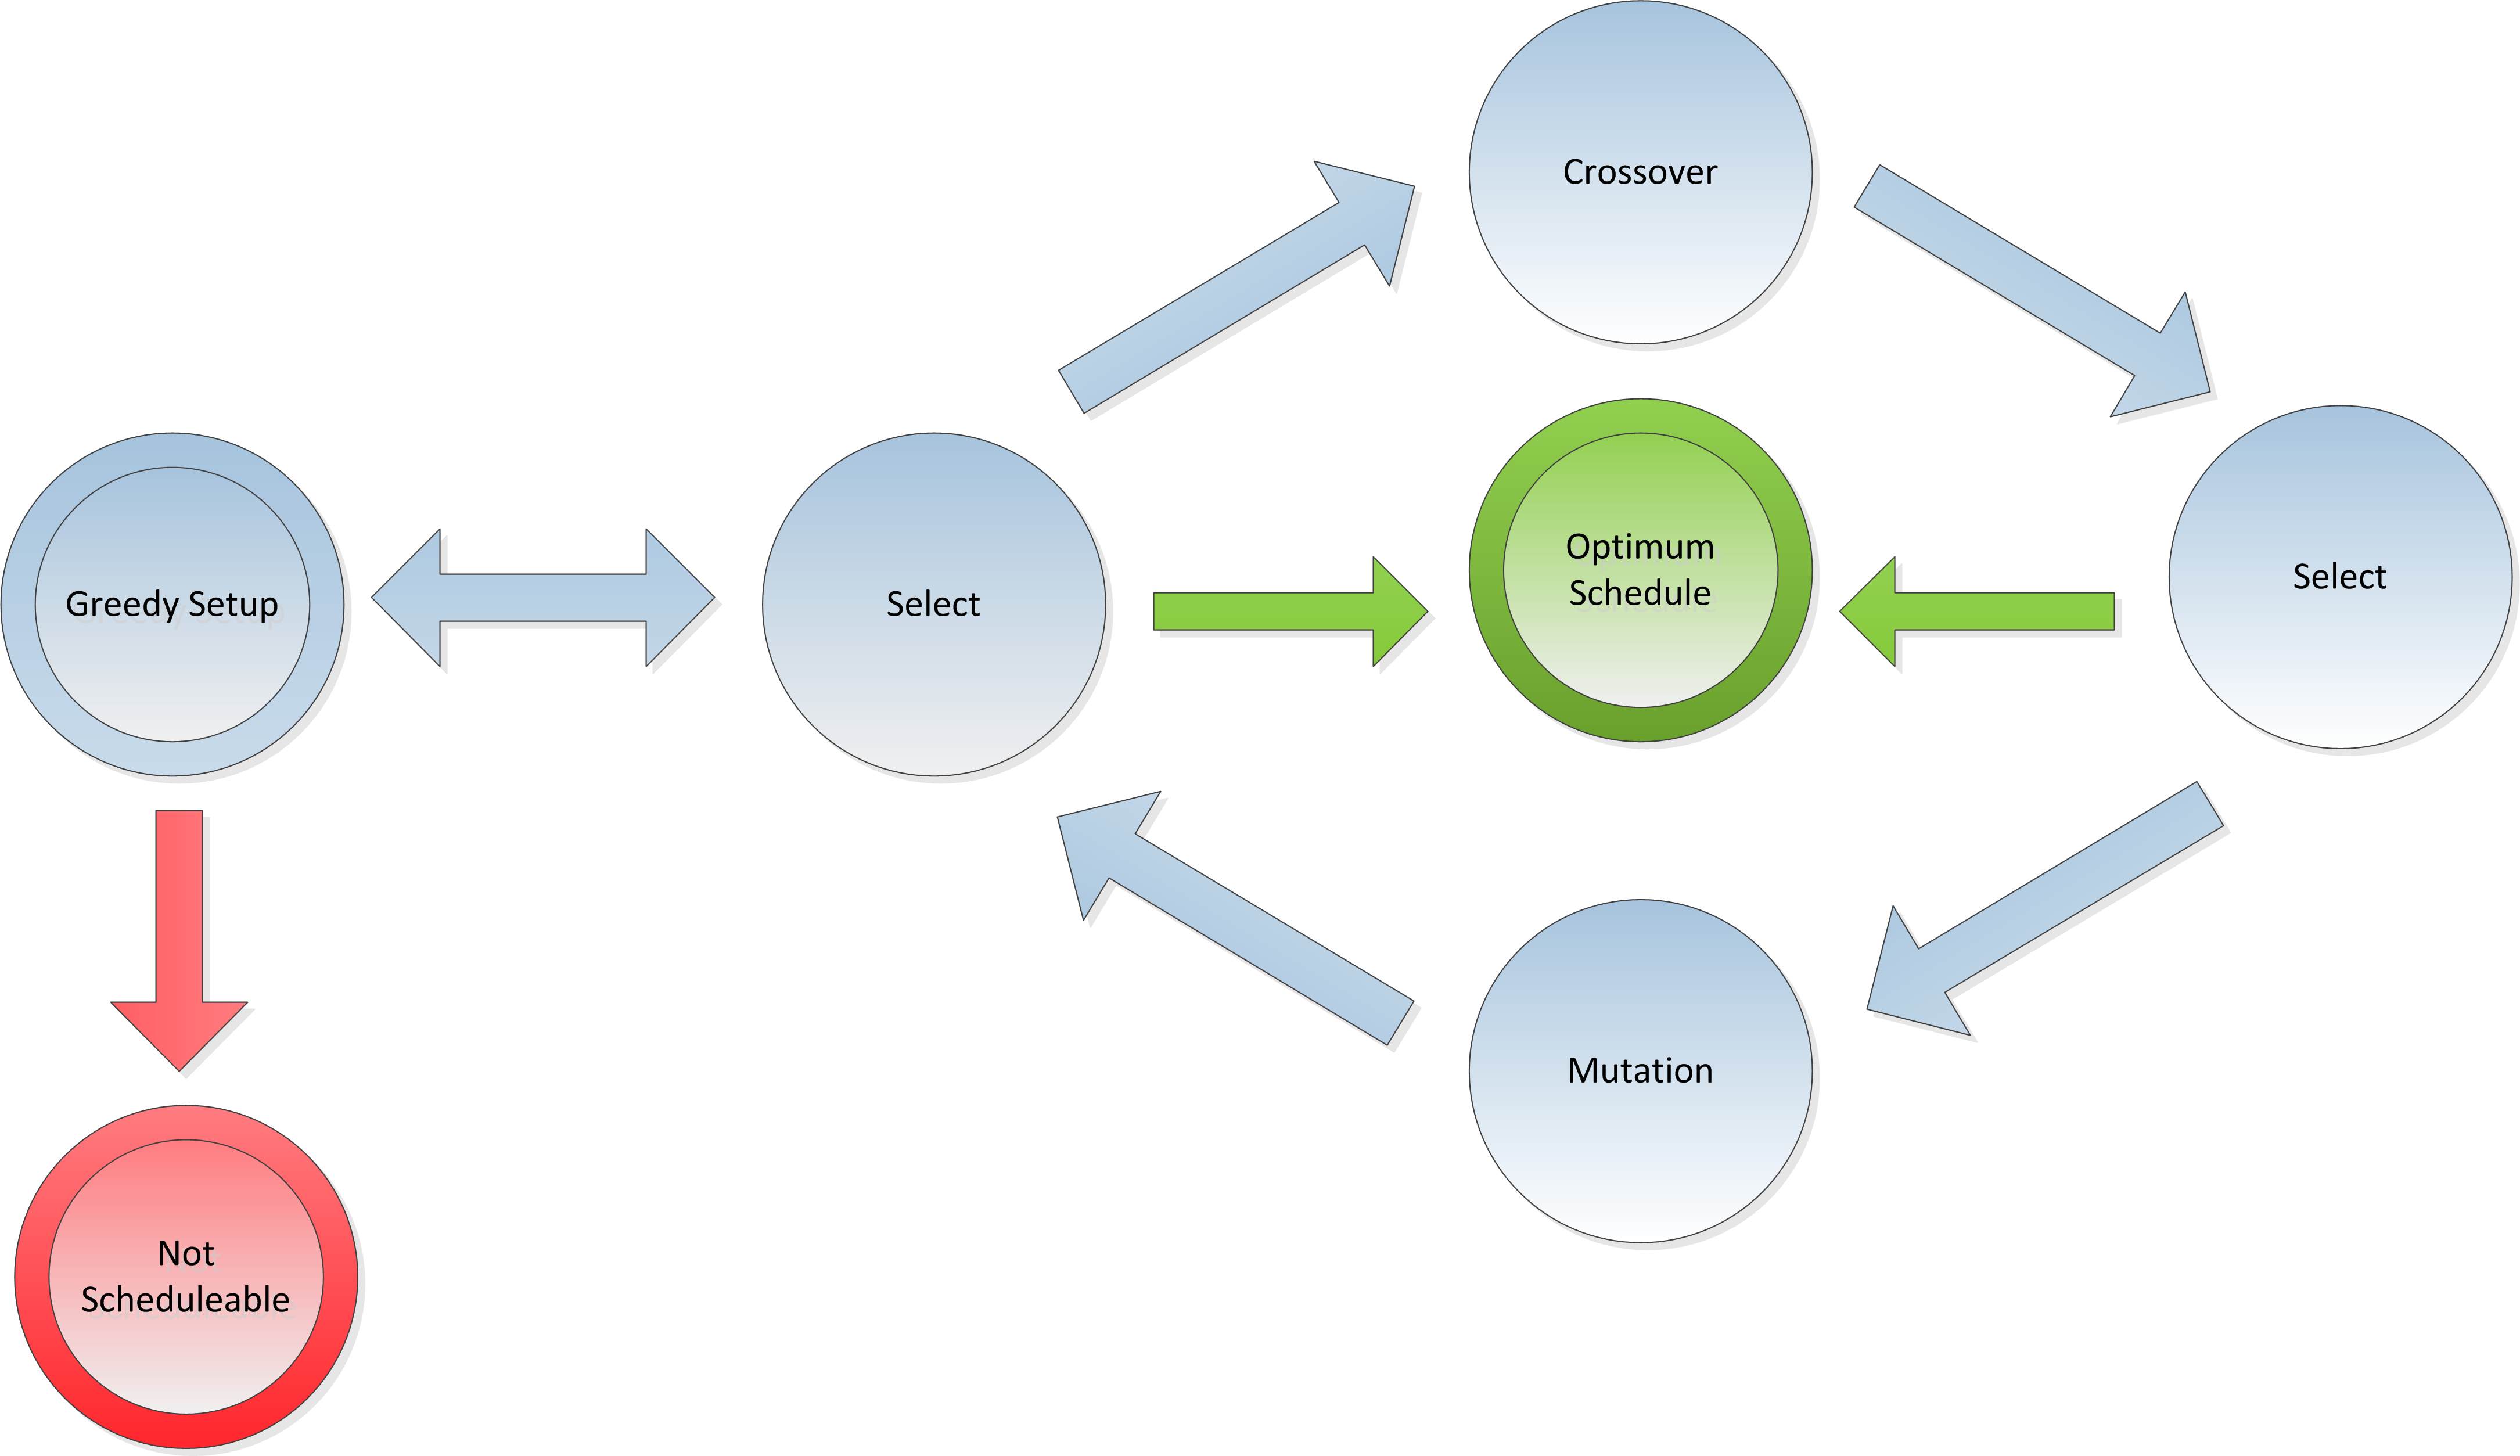
\includegraphics[width=\textwidth]{images/scheduler.png}
	\caption{Routine of the scheduler algorithm. Greedy Setup generates a initial population of candidate solutions. Every candidate solution is scored. If non-solvable conflicts appear the scheduling has to be terminated by means of not being scheduleable. Otherwise the Setup phase is followed by optimizing the candidate solutions by applying crossover and mutation operation until an optimum schedule is found.}
	\label{fig:scheduler}
\end{figure}

There is the possibility of finding an optimal solution in the phase of \emph{Greedy setup}. Therefore the \emph{fitness function} is applied on every generated candidate solution. If a optimal schedule was found the algorithm has terminated.


It is also possible the wished scheduling is not scheduleable at all. For instance when two course have the hard constraint to be placed at the same room with overlapping time. In this case the scheduling is stopped and the user has to resolve the constraint conflict by himself.

Otherwise the \emph{Greedy setup} will complete and the iteration of applying \emph{crossover}, \emph{mutation} and \emph{select} operation is started.  After each \emph{crossover} and \emph{mutation} only the best $\mu$ candidate solutions are kept and are tested for reaching the score $1.0$ which would lead to the algorithm termination.


\section{Technologies}
The following sections will discuss the technologies used in our project and the rationale behind them. For each technology we state the software or tool we used.

\subsection{Programming languages}
\begin{description}

\item[Java] is the only language that all members had a reasonable level of skill in. Thus it was preferred over other languages such as Haskell, PHP, Python. Perl and Ruby. We did however not restrict ourselves to using only Java but instead employed AspectJ which is described in the next paragraph.

\item[AspectJ] as we were all familiar with Java and wanted to have aspects, which is especially useful to supplement auto-generated code. Regarding the amount of time spent to learn new technologies and the fact that we did not have much of a time buffer,  this was the right decision. Using AspectJ did not force anyone in our team to learn a new language but still provided powerful features that were utilized by some where useful. Especially considering the huge amount of auto-generated code, AspectJ was a great choice as it allowed us to plug in functionality in some auto-generated classes without changing the other auto-generated classes and also allowed do this in a most simple way.

\item[PL/pgSQL] as we wanted to take advantage of the performance of Postgres for some of our functions. We carefully examined functions that could be implemented in PL/pgSQL, to see if implementing it on application level might be better. Accordingly we are convinced that using PL/pgSQl in those cases that we did is beneficial to overall performance.

\item[Ant \& Shell scripts] were used for routinely operated jobs. As the amount of time to write a shell script is small they quickly payed of. 
\end{description}

\subsection{Tools}
\begin{description}

\item[Wikis] are often used to spread knowledge over a wide community, we also used a wiki. This way we had the possibility to work on all different documents that were important for the project, like various guidelines, usecases, reports of iterations. As well all member were able to enter their personal timetables of the week, so each of us could easily see when some of us were available. 

\item[Ticket system] was needed during the project, since we needed a system that could save all kinds of problems regarding the current implementation. As Mail is not the best way to do so, we installed a ticket system provided by \emph{trac}. Sadly it was rarely used in the first few iterations. But as the project went on, we realized that there were many situation when there was something missing or not working properly, so anybody could simply open a ticket, describe the problem, assign a component of the project, and even assign a person who's responsible for that certain problem. 

\item[Web-server] 

\item[Build tool] were often used, when several tasks are done various times, like compiling code or cleaning directories. As we used Java as mainlanguage for our project the decision to use \emph{ant} was pretty easy. Another reason for \emph{ant} is the fact, that we provide a mechanism to deploy our software easy and fast, since no additional software needs to be installed except for Java, which is required anyway.

\item[IDE] are also common for repeatative tasks but that was not a problem anymore, since we used other build tools. First of all, different people write different code and what we want is a homogenous product, both the application the user is confronted with and the underlaying code. So we decided to use \emph{Eclipse} as our IDE, which will autoformat code with a given stylesheet. This way the code will always have the same look and feel. Secondly it's important to not think about missing code and the fact we used AspectJ could have been problematic. Luckily \emph{Eclipse} will automatically combine sourcecode from Java with the code from AspectJ so you don't have worry about missing functions while writing the code.

\item[JUnit]

\item[DBMS] as we needed a way to save our data persistent for both the scheduler and the web user interface. One goal was to use FLOSS as much as possible \emph{PostgreSQL} seemed reasonable for us, since some of us already used it succesfully on smaller projects.

\item[CVS] are very useful for larger projects with more than one person working on the code. With common sense you realize that it's impossible to review every code from other members to combine them seperatly or even the consistent spreading of code to others is nearly impossible. As there are several CVS that pretty much offer the same, we come to a decision to use \emph{subversion}, because our institute provided already \emph{subversion} for other students, so no time was wasted on configurating our own \emph{subverison}. 
\end{description}


\subsection{Relational model}



\section{Implementation}

\subsection{Scheduler}

The scheduler was implemented as backend of our application and was therefore a core component. After researching possible implementation approaches we decided to implement the basic structure of the scheduler in pair programming. We expected this decision will result in a  well-conceived design and basic implementation. The second reason was two have at least two team members being knowledgeable of this component.

\vskip 2ex

A lot of effort was spent into the implementation of the data-structure modeling a possible schedule solution in order to apply the genetic algorithm in an efficient way. Genetic algorithms operation are based on a data-structure which enables them to be applied. \emph{Crossover} and \emph{Mutation} need properties which can be manipulated.

\vskip 2ex

For these reasons a \emph{Map} was used.

\[Course \mapsto (Room,Time Slot)\]

Applying \emph{Crossover} and \emph{Mutation} means to take direct affect on this map. However this \emph{Map} serves only as an access for the genetic algorithm. Behind it is the data-structure modeling the actual schedule. A \emph{List} of rooms, each having a separate \emph{List} of time slots. Further each time slot has a \emph{List} of Courses as random factors of our algorithm rise possibility having two course at the same time in the same room. This data-structure is illustraed in the following figure:


\section{Verification and Validation}

This section will cover testing and other measurements which were taken to convince ourself of the correctness of our implementations. But also performance measurement is part of Verification and Validation.

\subsection{JUnit}

\subsubsection{Scheduler Validation}

Testing the scheduler for correctness is a non-trivial task. Not only raises the presents of a genetic algorithm the complexity, but also does its random-factor make it hard to test conditions which have to be satisfied all the time.

One approach to improve the testability of the scheduler is the introduction of a seeded random generator. Whenever randomness is applied in the scheduler, it can be reproduced by using the same seed.

In order to achieve a high guarantee of the schedulers correctness JUnit tests were implemented as little as possible. There are unit tests for every component of the scheduler, for instance a unit test testing the \emph{crossover} operation. On the downside unit tests allow only little input testing. Data-driven testing would be a more promising approach for testing the scheduler. On the other side this makes it also harder to check for correctness.

\subsection{Performance}

Performance, especially of the scheduler, can be easily tested by test runs with varying size of data input. However this gives no detailed information about the actual performance of separate components. For that reason the profiler \emph{JProfiler} was used to inspect the Java Virtual Machine while executing the program. This lead to a step-by-step process of picking up the slowest component display in the profiler and trying to improve its performance. In some cases this procedure gave us huge performance boosts.


\section{The Application}

\emph{Description of our product. Features and the concept behind the UI. Possible improvements and add-ons.}

\subsection{Usability}

MyCourses is able to create a semi-automatic scheduling for programs at universities or schools. It can also provide a scheduling that was run fully-automatic but the recommended usage is to have MyCourses create preliminary versions of a scheduling. These will then be improved by the users via the functionality for collaborative scheduling also provided by MyCourses. This process is best used iterative through several cycles of automatic assignment and manual improvement. To get better results from the automated scheduling users can define requirements and assign those to courses or resources. A requirement that is assigned to a course is regarded as a constraint that either must be met in case of a so called hard-constraint or simply improves the rating of a scheduling in case of a soft-constraint.

In Furthermore MyCourses provides functionality to

\begin{itemize}
\item enrol in courses

\item view your own schedule

\item view schedule for a room

\item import and export data

\item create, read, delete and modify data related to schedules
\end{itemize}


\section{Outcomes and lessons learned}
\subsection{Outcomes}
\emph{I dont know wether this should be located here or is intended to be somewhere else}
The web-application we have developed has some limitations due to different reasons \textsl{reasons to come}. It does not do this and that and another feature we should have implemented is not functional at the moment. The features should be easy to add, because they were considered during system design and no interface changes have to be made.

Beside our final application we also produced some side products which are worth to be mentioned. These include but are not limited to:
\begin{itemize}
	\item junction
	\item bakery
	\item weave
	\item lego
\end{itemize}
\emph{to be explained asap (as short as possible) by someone who knows how to do that}

Additionally we produced a large amount of project- and other documentation. (Details here)

\subsection{Lessons learned}
%\emph{What each of us had learned technology wise and what we have learned about projects.}
For all of us this was the first project of this size and duration. We took the chance to put into practice what we had learned in our software engineering course. Especially things that are not applicable for smaller projects. Things like (list of things).

We had to learn, that project-oriented approaches are hard to adhere to in an educational setting. Our team could not meet as often as claimed by nearly all development methods. Nevertheless we managed to establish a systematic meeting shedule.

At the beginning the proposed architecture of our software changed often and radical. Even with a given set of written down requirements. This was due to hard to understand requirements. There where different interpretations of the described requirements. We got it right after the first phase mainly because of (why?).

Our present team had not worked together previous to this project. We experienced that we are very different people with different approaches to problems. Near to the end of this project we are all friends and doing stuff together in our freetime. Everyone learned to get along with the originalities of the others. We have to highlight, that respect and honesty are very important in a team to lead to a productive development environment.
%this project resulted in a lot of valuable experience on how to work in a team
%And with mutual cooperation, understanding, respect and helping each other, we successfully overcome all problems.

We had to undergo the experince, that a complex development environment has to be easy to set up. Otherwise it will consume a lot of time even after small changes to get ready to work again.
%By  self  learning,  knowledge  sharing  and  organizing  sessions  on  various  technology related issues we led our development process in a smooth and systematic manner.
%Moreover, there was less time for testing of project.

During  the  project  we  have  a  good  chance  to  learn  some  new  technologies
List of things we learned stated by the team members:
\begin{itemize}
	\item XML
\end{itemize}

\section{Conclusion}

\emph{A short summary repeating the process, and the product.}

%\hrulefill

%Our project “Distributed Polling System” is a huge learning experience for us that has taught us to invest more time in proper architecture designing which in-turn reduces heavily the implementation time for any system. In addition to that, the architecture has guided us to segregate the whole system into  granular components that has enriched maximum re-usability and utmost team activity. Even the architecture has  helped  us  to  invest  less  time  for  component  integration  which  has  become evident  while  we started getting expected system behavior after our first time component assembling.

%In spite of having six team members from different cultural background and practices, by investing twenty  hours  per  person  per  week  for  almost  ten  weeks,  we  successfully  designed,  developed, integrated and tested the functionalities. It’s our honor and privilege to be part of such kind of  real time project implementation and we believe we could do further enhancement to this software in different aspects to make it a commercial software.

%Although  we  could  not  invest  much  more  time  due  to  having  parallel  courses  in  the  same curriculum,  we  would  be  grateful  to  work  further  on  this  software  to  make  it  commercially successful.

%\hrulefill

%This  project  was  done  in  a  quite  short  period  with  an  intensive  workload  (being  that  it  covers  half  university semester), nevertheless we profuse a lot of effort to provide a quality software. We reach this target working day by day, and through iterations in weekly periods and making different level of tests, both during programming and after deployment. We worked adding modules as “services” iteratively, to have always a working and testable version  since  the  first  ones.  We  also  divided  the  project  in  layers  to  make  each  part  as  more  independent  as possible. 

%Six people were involved in this work, from three different countries and belonging to two different universities, who have had different background and knowledge. The first part of project was the hardest because we had to work  hard  to  line  up  all  the  members.  After  that  we  proceeded  quicker  in  creating  the  software  and documentation to make the website easy to use (available to all kinds of people, with different requests). During all  the  developing  process  we  focused  on  making  the  product  extensible  and  ready  to  new  technologies,  like mobile phones.  

%The experience was great for all of us, we learned how to work in team in spite of distance and other working problems,  and  we  also  found  some  friends  more  than  co-workers.  Software  we  produced  is  already  being recognized  by  the  users,  and  with  only  a  few  days  passed  of  spreading  our  word  of  its  existence,  we  gathered many advices to our database. We have given users a great amount of freedom in structuring their advices which can  be  polygons,  lines  or  dots  and  contain  multimedia  information  and  links  to  relevant  advice  Web  page. Administration allows infinite number of advice categories and properties to be added, and with our promotion system, many users can become administrators or moderators thus making information more reliable and useful. 




\nocite{*}
\bibliographystyle{plain}
\bibliography{summary_report}



\end{document}
